\documentclass[12pt]{article}

\usepackage{sbc-template}
\usepackage{graphicx,url}
\usepackage[utf8]{inputenc}
\usepackage[brazil]{babel}
\usepackage{minted}
\usepackage[num]{abntex2cite}
\citebrackets[]
\sloppy

\title{Análise Empírica de Algoritmos de Ordenação}

\author{Douglas Juares Ortlieb\inst{1} \inst{2}}

\address{Universidade Tecnológica Federal do Paraná (UTFPR)\\
  Caixa Postal 271 -- 87301-899 -- Campo Mourão -- PR -- Brasil
\nextinstitute
  Departamento de Ciência da Computação (DACOM)
  \email{ortliebd@alunos.utfpr.edu.br}
}

\begin{document} 

\maketitle

\begin{abstract}
  This paper introduce the empirical analysis of the foremost sorting algorithms, the maximum subarray problem -- by recursive implementation -- and the binary search algorithm. Comparing the achieved results with the expected behavior given by asymptotic analysis of the same, lastly, does a comparation between the execution time of the sorting algorithms.
\end{abstract}
     
\begin{resumo}
  Este artigo apresenta a análise empírica dos principais algoritmos de ordenação, do problema da busca do subvetor máximo -- utilizando implementação recursiva -- e do algoritmo de busca binária. Comparando os resulados obtidos com o comportamento esperado dado pela análise assintótica dos mesmos, por fim, faz uma comparação entre o tempo de execução dos algoritmos de ordenação.
\end{resumo}

\section{Introdução} \label{sec:introducao}
Um algoritmo é qualquer procedimento computacional bem definido que toma algum valor ou conjunto de valores como entrada e produz algum valor ou conjunto valores como saída \cite{cormen:01}.

O problema de ordenação pode ser descrito como uma sequência de entrada $\langle a_1, a_2, \ldots, a_n\rangle$ que após a permutação dos elementos gera uma saída $\langle a_1^{'}, a_2^{'}, \ldots, a_n^{'}\rangle$ tal que $a_1^{'}\leq a_2^{'}\leq, \ldots, \leq a_n^{'}$ \cite{cormen:01}.

O problema de encontrar um subvetor máximo pode ser descrito como, dado um vetor com $n$ números inteiros (positivos e negativos) $V[1...n]$, encontre $V[e...d]$ tal que $e \geq 1$ e $d \leq n$ de maneira que $\sum_{i=e}^{d}V[i]$ é máxima \cite{foleiss:01}.

O problema de busca consiste em encontrar um valor, dado um vetor, cujo elemento seja igual a um valor informado.

Analisar a eficiência dos algoritmos torna-se necessário para compreender os recursos computacionais e o tempo gastos para sua execução, alguns problemas apresentam diversas soluções, a análise permite a escolha do algoritmo mais apropriada para determinada aplicação.

\subsection{Objetivos}
O objetivo principal deste trabalho é analisar empiricamente o tempo de execução de diversos algoritmos de ordenação e comparar o desempenho entre eles, bem como analisar o desempenho do algoritmo de busca binária e do algoritmo para encontrar o subvetor de soma máxima.

%%% Local Variables:
%%% TeX-master: "Artigo"
%%% End:
\section{Metodologia} \label{sec:metodologia}
A metodologia deste trabalho consistiu na implementação e análise do tempo de execução de sete algoritmos de ordenação, sendo eles: bubble sort, bubble sort com otimizações, insertion sort, selection sort, merge sort, heap sort e quick sort, um algoritmo de busca binária e um algoritmo para a busca do subvetor máximo, todos escritos em linguagem C++.

Para os algoritmos de ordenação e busca do subvetor máximo foram utilizados onze conjuntos distindos e aleatórios de dados classificados pelo tamanho -- 10 mil, 100 mil, 200 mil, 300 mil, 400 mil, 500 mil, 600 mil, 700 mil, 800 mil, 900 mil e 1 milhão de elementos -- todos do tipo inteiro e com valores contidos entre $[-999, 999]$.

Para o algoritmo de busca binária, foram utilizadas as mesmas entradas anteriores, porém ordenadas, o algoritmo foi executado cinco vezes para cada entrada e os dois maiores e menores valores foram descartados, os elementos chave para a busca também foram gerados de forma aleatória e estavam contidos entre $[-1999, 1999]$, permitindo assim, que valores não existentes nos vetores fossem pesquisados.

Para medir o tempo de execução de cada algoritmo foi utilizada a função \textit{clock\_t clock (void)} presente na biblioteca \textit{time.h}\footnote{Disponível na linguagem C e C++} e o macro \textit{CLOCKS\_PER\_SEC}. A função foi chamada antes e depois do algoritmo analizado, calculando a diferença do tempo final menos o tempo inicial e dividindo pelo macro, obtemos o tempo de execução do algoritmo ou seja,
$(tempo_{final} - tempo_{inicial}) / CLOCKS\_PER\_SEC$.

Para calular o número de iterações realizadas por cada algoritmo, foi criada uma variável auxiliar e feito o seu incremento nos trechos mais significativos de cada código, ficando, de maneira geral, contida nos laços mais internos de cada funções.
\subsection{Experimentos}
Cada algoritmos de ordenação foi executado onze vezes com entrada de tamanhos diferentes, totalizando 110 execuções. O algoritmo de busca do subvetor máximo foi executado uma vez para cada uma das onze entras, totalizando 11 execuções. O algoritmo de busca binária foi executado cinco vezes para cada entrada, totalizando 55 execuções.

Para realizar o experimento foi utilizado um notebook com processador Intel Core i5-6200u 2.8 GHz, 12 GB de memória RAM com sistema operacional Manjaro Linux.\footnote{Versão do kernel: 4.14.78-1-MANJARO}
%%% Local Variables:
%%% TeX-master: "Artigo"
%%% End:
\section{Resultados} \label{sec:resultados}
Para calcular o tempo e o número de iteração de alguns algoritmos de ordenação utilizamos interpolação númerica, pois o tempo de execução estava levando mais de uma hora para entradas acima de quatrocentos mil elementos.

Como utilizamos entradas com valores aleatórios entre -999 e 999 o Quick Sort, com implementação do pivô fixo no último elemento, se mostrou um pouco ineficiente, pois durante a execução do particionamento caiu no seu pior caso. Entretanto para o Inserion Sort o comportamento foi o oposto, permitindo que o algoritmo apresentasse comportamento semelhante ao seu melhor caso. Para a Busca Binária, dada a frequencia com que os mesmos números apareciam nos vetores, o algoritmo apresentou comportamento $\Theta(1)$ para algumas entradas.

Os gráficos abaixo representam o tamanho da entrada pelo número de iterações necessárias para resolver o problema, comparando o resultado da análise empírica com a análise assintótica para o caso mais próximo apresentado.

\subsection{Bubble Sort}
O método do bubble sort consiste em mover os menores valores para o início e os maiores valores para o final da lista de elementos, passando diversas vezes pela lista e comparando os elementos adjacentes, caso estejam fora de ordem, serão trocados \cite{mcconnell:01}.

A ordem assintótica do algoritmo é $\Theta(n^2)$, pela análise empírica obtivemos uma expressão com o mesmo comportamento, porém com ordem de crescimento menor, como pode ser visto na Figura~\ref{fig:bubble}.
\begin{figure}[h]
\centering
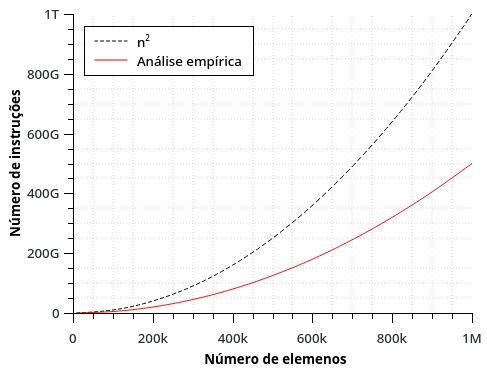
\includegraphics[scale=0.7]{images/bubble_graph.jpg}
\caption{Bubble Sort}
\label{fig:bubble}
\end{figure}

\subsection{Bubble Sort com otimizações}
Uma possível otimização para o bubble sort é atravez de uma condição de parada caso o laço interno não efetue nenhuma troca de elementos \cite{geeks:01}, quando isso ocorre significa que o vetor já está ordenado e a complexidade, para o melhor caso, passa a ser $O(n)$.

Para os casos testados, o decréscimo no número de instruções foi praticamente insignificante se comparado ao valor total. Fator facilmente observado na Figura~\ref{fig:bubble_optimized}, mostrando diferenças mínimas para o gráfico da Figura~\ref{fig:bubble}.
\begin{figure}[h]
\centering
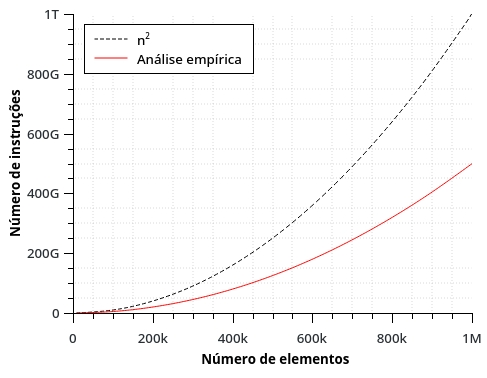
\includegraphics[scale=0.7]{images/bubble_optimized_graph.jpg}
\caption{Bubble Sort Otimizado}
\label{fig:bubble_optimized}
\end{figure}

\subsection{Insertion Sort}
A primeira iteração do algoritmo pega o segundo elemento do vetor e, se for menor que o primeiro elemento, troca-os de posição. A segunda iteração compara o terceiro elemento e o insere na posição correta de acordo com os dois primeiros elementos. Na $i^{n-ésima}$ do algoritmo, os primeiros $i$ elementos do vetor original estarão ordenados \cite{deitel:01}.

Possui complexidade $O(n^2)$ para o caso médio e o pior caso, para o melhor caso tem comportamento $\Omega(n)$. Pela análise empírica, Figura~\ref{fig:insertion}, apresentou ordem $O(nlog(n))$, pois as entradas utilizadas possuíam valores que se repetiam diversas vezes, facilitanto o algoritmo a encontrar posição correta dos elementos.

\begin{figure}[ht]
\centering
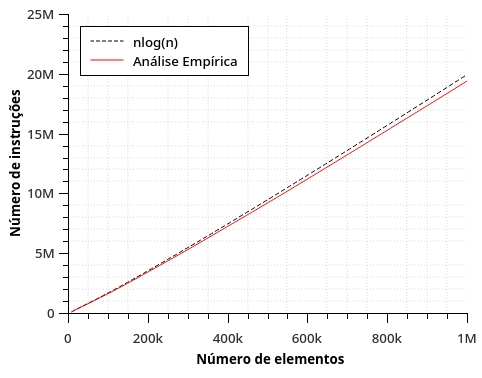
\includegraphics[scale=0.7]{images/insertion_graph.jpg}
\caption{Insertion Sort}
\label{fig:insertion}
\end{figure}
 
\subsection{Selection Sort}
A primeira iteração do algoritmo seleciona o elemento com menor valor e o troca com o primeiro elemento do vetor. A segunda iteração seleciona o segundo elemento com menor valor e o troca com o segundo elemento do vetor. O algoritmo continua até a útima iteração, onde seleciona o elemento com o segundo maior valor e o troca com o penúltimo elemento no vetor, deixando o maior valor no último elemento \cite{deitel:01}.

Possui ordem assintótica $\Theta(n^2)$ devido a laços invariantes, como pode ser observado pela análise empírica, Figura~\ref{fig:selection}.
\begin{figure}[ht]
\centering
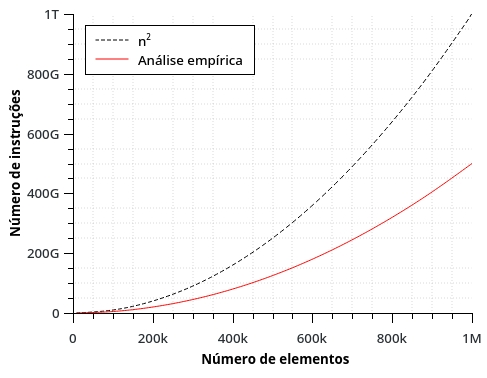
\includegraphics[scale=0.7]{images/selection_graph.jpg}
\caption{Selection Sort}
\label{fig:selection}
\end{figure}

\subsection{Merge Sort}
A ideía básica do algoritmo é ordenar um vetor dividindo-o em dois sub-vetores de mesmo tamanho até que cada sub-vetor tenha apenas um elemento, então ordena cada sub-vetor e os junta de volta, resultando em um novo vetor ordenado. Método conhecido como divisão e conquista.

Possui complexidade $\Theta(nlog(n))$ e pela análise empírica apresentou examente este comportamente, como pode ser visto na Figura~\ref{fig:merge}. 
\begin{figure}[ht]
\centering
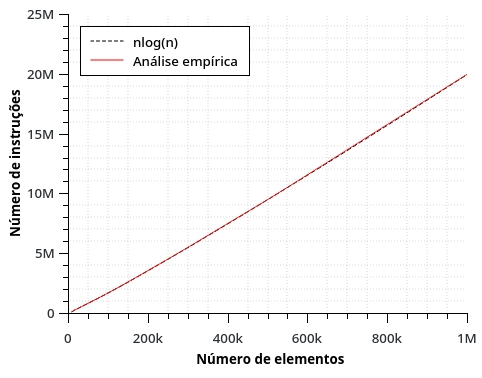
\includegraphics[scale=0.7]{images/merge_graph.jpg}
\caption{Merge Sort}
\label{fig:merge}
\end{figure}

\subsection{Heap Sort}
A idéia básica do algoritmo é transformar o vetor em uma estrutura de dados heap, a qual tem a propriedade de permitir, de forma eficiente, a obtenção e remoção dos elementos de maior valor. Repetidamente retirando o elemento de maior valor do heap e construindo o vetor ordenado do fim para o início \cite{rosetta:01}.

Possui complexidade $\Theta(nlog(n))$ para todos os casos, como também pode ser observado pela análise empírica, Figura~\ref{fig:heap}.
\begin{figure}[h]
\centering
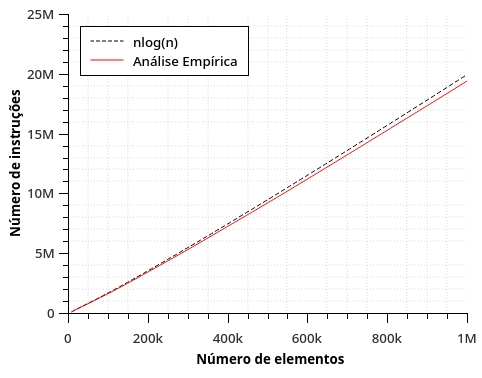
\includegraphics[width=0.7\textwidth]{images/heap_graph.jpg}
\caption{Heap Sort}
\label{fig:heap}
\end{figure}

\subsection{Quick Sort}
Assim como o Merge Sort, o Quick Sort também é um algoritmo de divisão e conquista. Ele seleciona um elemento como pivô e particiona os elementos de acordo com o valor do pivô, colocando os elementos menores a esquerda e os maiores a direita do pivô \cite{geeks:02}.

Apresenta complexidade $\Theta(nlog(n))$ para o caso médio, entretanto para o pior caso possui ordem assintótica $O(n^2)$, apesar disso, o quick sort com frequência é a melhor opção prática para a ordenação, devido aos fatores ocultos na notação $\Theta(nlog(n))$ serem bastante pequenos \cite{cormen:01}.
O principal determinante de um bom desempenho está na escolha do pivô, podendo ser:
\begin{itemize}
\item Sempre escolher o primeiro elemento como pivô.
\item Sempre escolher o último elemento como pivô. Utilizado na implementação para este trabalho.
\item Escolher um elemento aleatório como pivô.
\item Escolher o elemento do meio do vetor como pivô.
\end{itemize}

Durante a análise empírica apresentou comportamento $O(n^2)$, Figura~\ref{fig:quick}, por termos tomado o último elemento como pivô e pelo vetor a ser ordenado possuir muitos elementos de mesmo valor, tornando o particionamento ineficiente.

\begin{figure}[ht]
\centering
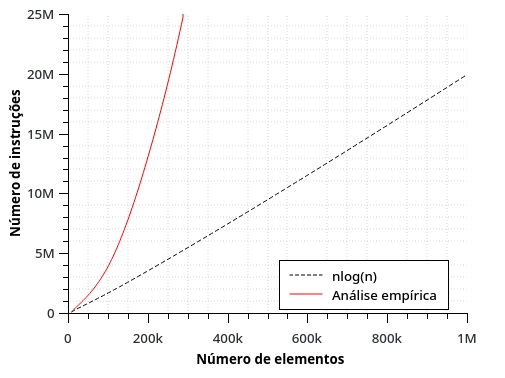
\includegraphics[width=.5\textwidth]{images/quick_graph.jpg}
\caption{Quick Sort}
\label{fig:quick}
\end{figure}

\subsection{Busca Binária}
Se nós compararmos o alvo com o elemento que está no meio de uma lista ordenada, teremos três resultados possíveis: encontramos o alvo, o alvo é menor que o elemento, ou o alvo é maior que o elemento. No primeiro e melhor caso, a busca está feita. Nos outros dois casos, sabemos que metade da lista pode ser elimida \cite{mcconnell:01}. O processo continua considerando apenas o vetor parcial onde o alvo pode estar localizado, terminando quando o vetor parcial possui apenas um elemento, ou quando o alvo é encontrado.

Sua complexidade é $O(log(n))$ e na análise empírica obtivemos exatamente isso em alguns pontos, em outros a podemos ver um comportamento constante, visto que o vetor ordenado de entrada possuia diversos entradas iguais, permitindo que o valor alvo fosse encontrado com facilidade, como pode ser observado na Figura~\ref{fig:busca}.
\begin{figure}[ht]
\centering
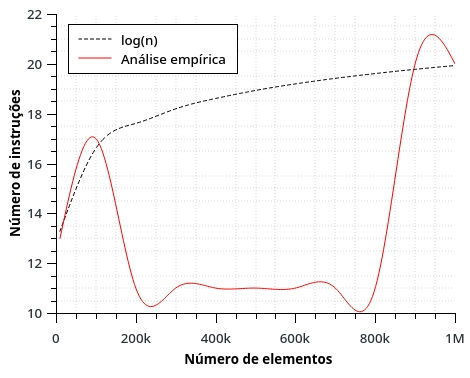
\includegraphics[width=.5\textwidth]{images/binary_graph.jpg}
\caption{Busca Binária}
\label{fig:busca}
\end{figure}

\subsection{Busca do Subvetor Máximo}
Queremos encontrar um subvetor máximo do subvetor $V[e...d]$. A divisão e conquista nos diz que devemos dividir o problema o mais igualitariamente possível, ou seja, podemos dividir ao meio, $m$, e considerar os subvetor $A[e...m]$ e $A[m + 1...d]$. Cada subvetor contíguo $A[i...j]$ em $A[e...d]$ deve estar em três lugares:
\begin{itemize}
\item inteiro no subvetor $A[e...m], e \leq i \leq j \leq m;$
\item inteiro no subvetor $A[m + 1...d], m \leq i \leq j \leq d, ou;$
\item entre $e \leq i \leq m \leq j \leq d$
\end{itemize}

Assim, o subvetor máximo $A[e...d]$ deve estar em um destes três lugares. De fato, um subvetor máximo de $A[e...d]$ deve ter a maior soma de todos os subvetor inteiramente em $A[e...m]$, inteiramente em $A[m + 1...d]$ ou cruzando $m$.

O algoritmo trabalha encontrando a maior soma do lado esquerdo do meio de $A$, $A[max-left...m]$ e a maior soma a partir do meio + 1 de $A, A[meio+1...max-right]$. Assim, o vetor máximo resultante é entre $A[max-left...max-right]$ \cite{foleiss:01}.

Apresenta complexidade $\Theta(nlog(n))$ e foi examente o que obtivemos através da análise empírica, como pode ser visto na Figura~\ref{fig:subvetor}.
\begin{figure}[ht]
\centering
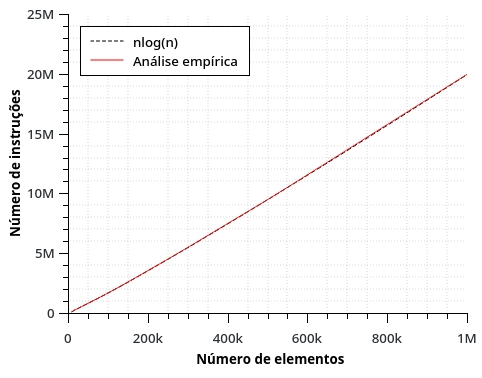
\includegraphics[width=.5\textwidth]{images/subvetor_graph.jpg}
\caption{Busca do Subvetor Máximo}
\label{fig:subvetor}
\end{figure}

%%% Local Variables:
%%% mode: latex
%%% TeX-master: "Artigo"
%%% TeX-command-extra-options: "-shell-escape"
%%% End:

\section{Análise dos Resultados e Conclusão}
Neste capítulo apresentaremos a comparação entre o tempo de execução dos algoritmos de ordenação e as concluções gerais sobre o projeto.

Na Tabela~\ref{tab:complexidade} podemos ver a complexidade dos algoritmos utilizados, como as
\renewcommand{\arraystretch}{1.5}
  \begin{table}[h]
    \centering
    \begin{tabular}[h]{|l|c|c|c|} \hline
      Algoritmo & Melhor caso & Caso Médio & Pior caso \\ \hline
      Bubble Sort & $\Omega(n^2)$ & $\Theta(n^2)$ & $O(n^2)$ \\ \hline
      Bubble Sort com otimização& $\Omega(n)$ & $\Theta(n^2)$ & $O(n^2)$ \\ \hline
      Insertion Sort & $\Omega(n)$ & $\Theta(n^2)$ & $O(n^2)$ \\ \hline
      Selection Sort & $\Omega(n^2)$ & $\Theta(n^2)$ & $O(n^2)$ \\ \hline
      Merge Sort & $\Omega(nlog(n))$ & $\Theta(nlog(n))$ & $O(nlog(n))$ \\ \hline
      Heap Sort & $\Omega(nlog(n))$ & $\Theta(nlog(n))$ & $O(nlog(n))$ \\ \hline
      Quick Sort & $\Omega(nlog(n))$ & $\Theta(nlog(n))$ & $O(n^2)$ \\ \hline
      Busca Binária & $\Omega(1)$ & $\Theta(log(n))$ & $O(log(n))$ \\ \hline
      Busca do Subvetor Máximo & $\Omega(nlog(n))$ & $\Theta(nlog(n))$ & $O(nlog(n))$ \\ \hline
    \end{tabular}
    \caption{Complexidade dos algoritmos analisados}
    \label{tab:complexidade}
  \end{table}
  entradas geradas para os problemas possuiam valores aleatórios, esperava-se que os algoritmos executassem para o caso médio, como foi para a maioria dos casos testados, entretanto o Insertion Sort executou com comportamento $nlog(n)$, variando entre o pior e o melhor caso, pois como a entrada continha diversos elementos repetidos, era possível encontrar com facilidade a posição correta para a inserção dos elementos.

  O Quick Sort, contudo, variou entre o caso médio e o pior caso, com o pivô fixo na última posição e muitos valores repetidos, o algoritmo não se mostrou eficiente durante a fase do particionamento, gerando uma árvore de recursão desbalanceada, porém ele ainda se mostrou mais eficiente que os algoritmos que executam em $n^2$.

  Para o algoritmo de Busca Binária, o fator da repetição dos números também influenciou no resultado final, podemos observar o algoritmo apresentando comportamento $\Theta(1)$. Mesmo quando o algoritmo caiu no seu pior caso, buscar um elemento cujo valor não está contido no vetor, seu tempo de execução continua ótimo, independente do tamanho da entrada.

  Na Figura~\ref{fig:eficientes} podemos ver o comparativo entre os tempos de execução dos algoritmos de ordenação que se mostraram mais eficientes na resolução do problema,
\begin{figure}[ht]
\centering
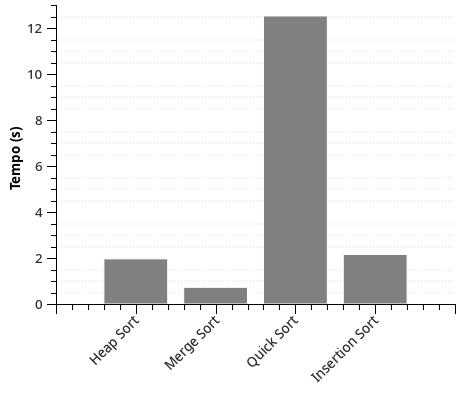
\includegraphics[scale=0.9]{images/eficientes_graph.jpg}
\caption{Algoritmos eficientes durante a análise empírica}
\label{fig:eficientes}
\end{figure}
o Merge Sort se mostrou mais eficiente, seguido pelo Heap Sort e o Insertion Sort, entretanto devemos enfatizar que o Insertion Sort é considerado um algoritmo de ordenação ineficiente, pois como sabemos, um algoritmo tem maior chance de executar com comportamento tendendo ao caso médio e que o caso médio costuma ser tão ruim quanto o pior caso.


Na Figura~\ref{fig:ineficientes} vemos o tempo de execução para os algoritmos ineficientes, 
\begin{figure}[ht]
\centering
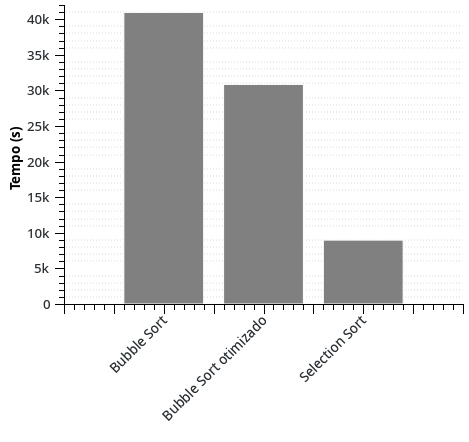
\includegraphics[scale=0.9]{images/ineficientes_graph.jpg}
\caption{Algoritmos ineficientes durante a análise empírica}
\label{fig:ineficientes}
\end{figure}
o Bubble Sort apresentou uma melhora significativa, contudo, ainda longe de tornar o algoritmo utilizável para a resolução de problemas com entradas muito grandes, sendo que a partir de quinhentos mil elementos, ele leva cerca de duas horas para finalizar o processo. O Selection Sort, apesar de realizar o mesmo número de instruções que o Bubble Sort, conseguiu executar em um tempo muito menor.
%%%Local Variables:
%%% TeX-master: "Artigo"
%%% End:

\bibliographystyle{abntex2-num}
\bibliography{referencias}

\end{document}